\label{ch:incompressible}

\begin{quote}
\noindent {\em These summarize methods for solving the incompressible
  hydrodynamics equations using an cell-centered approximate
  projection method.}
\end{quote}

\section{Incompressible flow}

As a fluid parcel advects through a domain, it compresses and expands
due to a variety of effects (stratification, local heat release,
acoustic/shock waves).  The Lagrangian derivative of the density
captures the changes in the fluid, and is a measure of its compressiblity.
From the continuity equation, we see:
\begin{equation}
-\frac{1}{\rho}\frac{D\rho}{Dt} = \nabla \cdot U
\end{equation}
Note that for $\nabla \cdot U > 0$, we have $-(1/\rho) (D\rho/Dt) > 0$,
which means that $\rho$ gets smaller---this is expansion of the Lagrangian
fluid element.

A fluid in which the density (and therefore volume) of a fluid element is not
allowed to change is called {\em incompressible}.  An incompressible
fluid obeys the velocity constraint:
\begin{equation}
\nabla \cdot U = 0
\end{equation}
(since $D\rho / Dt = 0$).  The incompressible fluid approximation is 
a reasonable approximation when the Mach number of the fluid is small
($\ll 1$).  To complete the system, we add the momentum equation.  If 
we take the density to be constant everywhere in the domain (not just
in our fluid element), then we have:
\begin{equation}
\frac{\partial U}{\partial t} + U \cdot \nabla U + \nabla p = 0
\end{equation}
Note that $p$ here looks like a pressure, but it is not subject to
any equation of state.  This system is closed as written.  The value
of $p$ is determined such that the velocity constraint is satisfied.



\section{Projection methods}

The basic idea behind a projection method is that any vector field
can be decomposed into a divergence free part and the gradient of 
a scalar (this is sometimes called a {\em Hodge decomposition}).  
Given a velocity field $U^\star$, we can express it in terms of the 
divergence free part $U^d$ and a scalar, $\phi$ as:
\begin{equation}
U^\star = U^d + \nabla \phi
\end{equation}
Taking the divergence of each side, and noting that $\nabla \cdot U^d
= 0$, we have
\begin{equation}
\nabla \cdot U^\star = \nabla^2 \phi
\end{equation}
This is an elliptic equation.  Given suitable boundary conditions, we
can solve for $\phi$ (for instance, using multigrid) and recover the
divergence free part of $U^\star$ as:
\begin{equation}
U^d = U^\star - \nabla \phi
\end{equation}
We call this operation of extracting the divergence free part of a
velocity field a {\em projection}.  This can be expressed by defining
an operator $P$, such that $PU^\star = U^d$, and $(I - P)U^\star =
\nabla \phi$.  From the momentum equation, we see that $\partial
U/\partial t + \nabla \phi$ is in the form of a divergence free term
$+$ the gradient of a scalar.  This means that advancing the velocity
field subject to the constraint involves solving:
\begin{equation}
U_t = P(U_t + \nabla p) = P(-U\cdot \nabla U)
\label{eq:projevolve}
\end{equation}
See Bell, Colella, and Howell~\cite{BCH} for a nice discussion of this.

The original projection method for incompressible flows goes back to
Chorin~\cite{chorin:1968}.  Instead of evolving
Eq.~\ref{eq:projevolve} directly, we break the update into pieces.
The basic idea is to evolve the velocity advection equation without
regard to the constraint, yielding a {\em provisional velocity} field
which is then subjected to a projection to enforce the divergence-free
constraint.  Bell, Colella, and Glaz (BCG)~\cite{BCG} introduced a projection
method that uses standard Godunov methods for the advection terms
(much like is done with compressible flow) and then solves an elliptic
equation to enforce the constraint.  This division of the operations
in the algorithm (advect then project) is a type of {\em fractional
  step} method.

There are different ways to discretize the operators that make up the
projection.  We denote the discretized divergence as $D$ and the
discretized gradient operation as $G$.  For an exact projection, the
discretized Laplacian, $L$, would be the same as applying $G$ and $D$
in succession (i.e. $L = DG$).  Depending on our data centerings, we
may prefer to discretize the Laplacian independently to $D$ and $G$,
such that $L \ne DG$.  This is called an {\em approximate projection}.
Note that for an approximate projection, $P$ is not
idempotent: $P^2 U \ne PU$.

Many variations on this basic idea exist, using alternate forms of the
projection, different grid centerings of the $\phi$ variable, and
additional physics.


\section{Cell-centered approximate projection solver}

Here we describe an incompressible algorithm that uses cell-centered
data throughout---$U$ and $p$ are both cell-centered.  The
projection at the end is an approximate projection.  The basic
algorithm flow is 
\begin{itemize}
\item Create the time-centered advective velocities through the faces
  of the zones.
\item Project the advective velocities such that they obey the
  velocity constraint
\item Construct the time-centered interface states of all quantities
  on the faces of the zones using the advective velocity.
\item Update the velocity to the new time.  This is defines the
  provisional velocity field---it does not yet satisfy the constraint.
\item Enforce the velocity constraint by projecting the velocity.
\end{itemize}

The description below is pieced together from a variety of sources.
BCH describes a cell-centered method, but with an exact projection
(with a larger, decoupled stencil).  Almgren, Bell, and Szymczak
(ABS)~\cite{ABS} describes an approximate projection method, but with
a node-centered final projection.  We follow this paper closely up
until the projection.  Martin and Colella~\cite{MartinColella} (and
Martin's PhD thesis) method uses a cell-centered projection, as is
described here.  They go into additional effort to describe this for a
refined grid.  All of these method are largely alike, aside from how
the discretization of the final projection is handled.

\subsection{Advective velocity}

In predicting the interface states, we first seek to construct the
velocities through the interfaces.  A key concept throughout the
advection step is that once we have the normal velocities on the
interfaces, we can use these to upwind left and right states of any
quantity to get their interface value.  The advective velocities we
construct here, ${u}^\mathrm{adv}$ and ${v}^\mathrm{adv}$,
will later be used to upwind the various states we predict to the
interfaces.  We only need the velocity through the interfaces, as
shown in the figure \ref{fig:MAC}. This staggered grid arrangement is
sometimes called a MAC grid.

\begin{figure}[h]
\centering
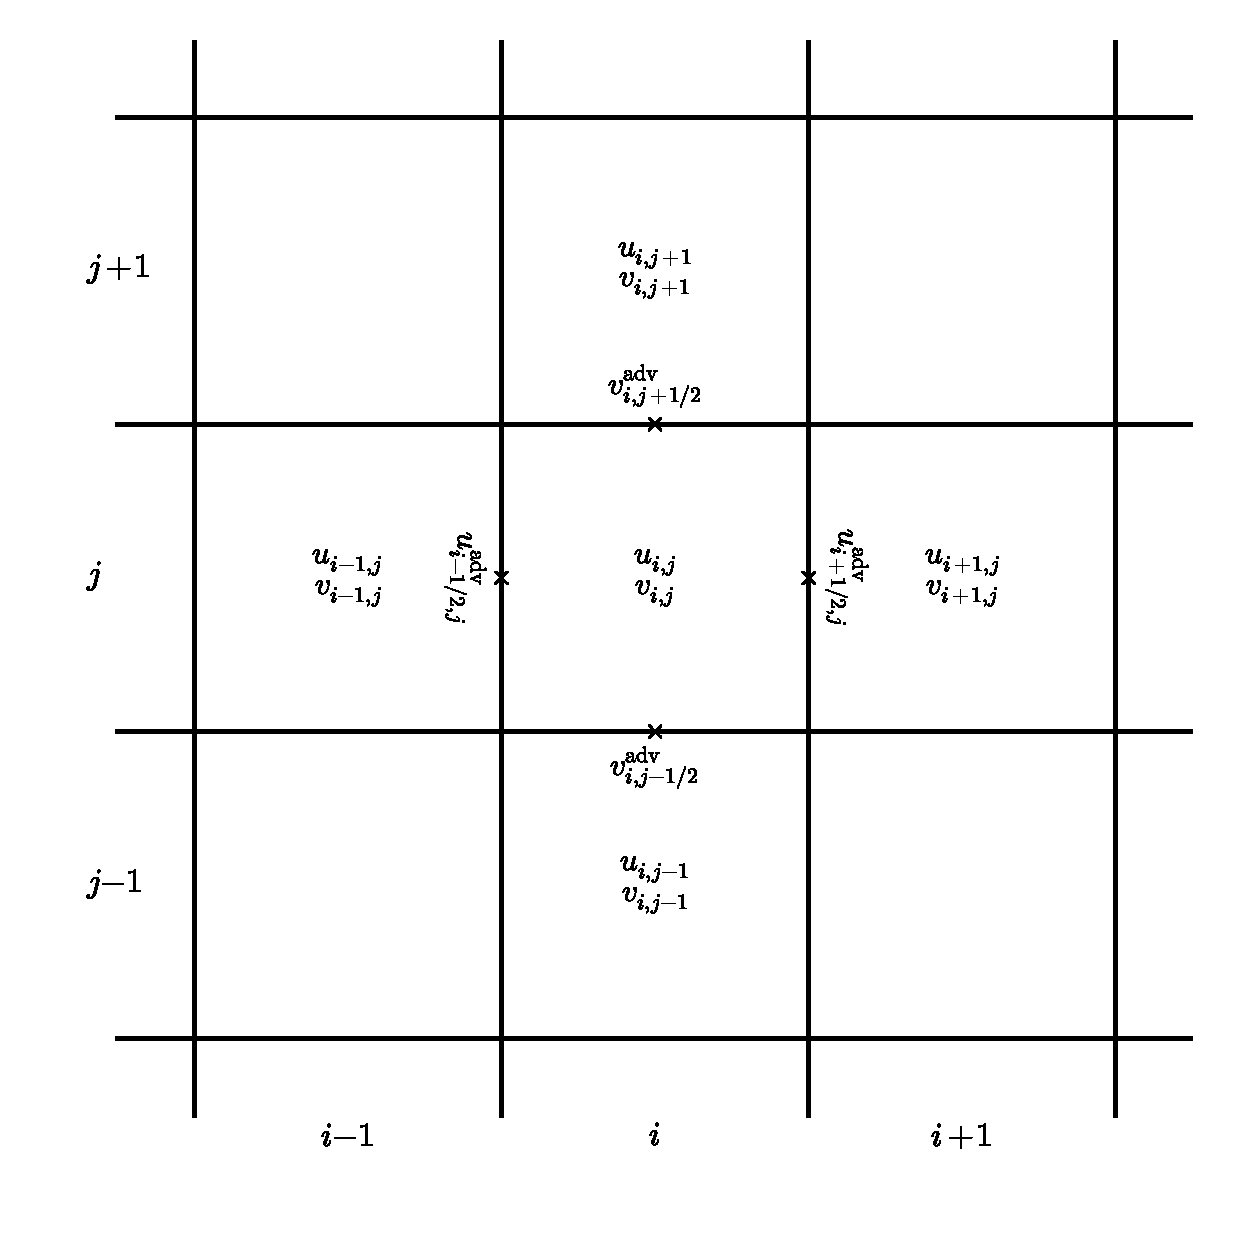
\includegraphics[width=3.3in]{MAC}
\caption{\label{fig:MAC} The staggered `MAC' grid for the advective
  velocities}
\end{figure}


We follow ABS.  Our velocity evolution system (writing out the
individual components of $U$: $u$ and $v$) is
\begin{eqnarray}
\frac{\partial u}{\partial t} &=& -u \frac{\partial u}{\partial x} 
                                  -v \frac{\partial u}{\partial y} 
                                  -\frac{\partial p}{\partial x} = 0 \\
\frac{\partial v}{\partial t} &=& -u \frac{\partial v}{\partial x} 
                                  -v \frac{\partial v}{\partial y} 
                                  -\frac{\partial p}{\partial y} = 0 
\end{eqnarray}
Our goal in this step is to predict time-centered interface values of
the normal velocity ($u$ on x-edges and $v$ on y-edges).  The
prediction follows from Taylor expanding the state to the interface
(through $\Delta x/2$ or $\Delta y/2$) and to the half-time (through
$\Delta t/2$).  As with the regular advection, we can have left and
right states which we will resolve by solving a Riemann problem.  The
left interface state of $u$ at $i+1/2,j$ is found as:
\begin{eqnarray}
u_{i+1/2,j,L}^{n+1/2} 
  &=& u_{i,j} 
    + \frac{\Delta x}{2} \left . \frac{\partial u}{\partial x} \right |_{i,j}
    + \frac{\Delta t}{2} \left . \frac{\partial u}{\partial t} \right |_{i,j}\\
  &=& u_{i,j} 
    + \frac{\Delta x}{2} \left . \frac{\partial u}{\partial x} \right |_{i,j}
    + \frac{\Delta t}{2} \left . \left (-u \frac{\partial u}{\partial x}
                                -v \frac{\partial u}{\partial y}
                                -\frac{\partial p}{\partial x} \right ) \right |_{i,j}\\
  &=& u_{i,j} 
    + \frac{\Delta x}{2} \left ( 1 - \frac{\Delta t}{\Delta x} u_{i,j} \right )
                         \left .  \frac{\partial u}{\partial x}\right |_{i,j}
    - \frac{\Delta t}{2} \left ( v \frac{\partial u}{\partial y}\right )_{i,j}
    - \frac{\Delta t}{2} \left . \frac{\partial p}{\partial x} \right |_{i,j}\\
\end{eqnarray}
We express ${\partial u}/{\partial x} |_{i,j}$ as $\Dux_{i,j} / \Delta
x$, where $\Dux_{i,j}$ is the limited slope of $u$ in the
$x$-direction in zone $i,j$.  Our interface state is then:
\begin{equation}
u_{i+1/2,j,L}^{n+1/2} 
    = \underbrace{u_{i,j} + \frac{1}{2} \left ( 1 - \frac{\Delta t}{\Delta x} u \right ) \Dux_{i,j}}_{\equiv \hat{u}_{i+1/2,j,L}^{n+1/2}}
    - \underbrace{\frac{\Delta t}{2} \left ( v \frac{\partial u}{\partial y} \right )_{i,j}}_{\mathrm{transverse~term}}
    - \frac{\Delta t}{2} \left . \frac{\partial p}{\partial x} \right |_{i,j}
\label{eq:uMAC_l}
\end{equation} 


Similarly, for $v$ through the $y$ faces, we find:
\begin{equation}
v_{i,j+1/2,L}^{n+1/2} 
    = \underbrace{v_{i,j} + \frac{1}{2} \left ( 1 - \frac{\Delta t}{\Delta x} v \right ) \Dvy_{i,j}}_{\equiv \hat{v}_{i,j+1/2,L}^{n+1/2}}
    - \underbrace{\frac{\Delta t}{2} \left ( u \frac{\partial v}{\partial x} \right )_{i,j}}_{\mathrm{transverse~term}}
    - \frac{\Delta t}{2} \left . \frac{\partial p}{\partial y} \right |_{i,j}
\label{eq:vMAC_l}
\end{equation} 

As indicated above (and following ABS and the similar notation used by
Colella~\cite{colella:1990}), we denote the quantities that will be used to evaluate
the transverse states (consisting only of the normal predictor) with a
`$\hat{~}$'.  These will be used to evaluate the transverse terms
labeled above.

We predict $u$ and $v$ to both the $x$ and $y$ interfaces, using only
the normal part of the predictor.  This gives us the left and right `hat'
states on each interface.

\noindent $u$ on $x$-interfaces:
\begin{eqnarray}
\hat{u}_{i+1/2,j,L}^{n+1/2} &=&
   u_{i,j} + \frac{1}{2} \left ( 1 - \frac{\Delta t}{\Delta x} u_{i,j} \right )
       \Dux_{i,j} \\ 
%
\hat{u}_{i+1/2,j,R}^{n+1/2} &=&
   u_{i+1,j} - \frac{1}{2} \left ( 1 + \frac{\Delta t}{\Delta x} u_{i+1,j} \right )
       \Dux_{i+1,j} 
\end{eqnarray}

\noindent $v$ on $x$-interfaces:
\begin{eqnarray}
\hat{v}_{i+1/2,j,L}^{n+1/2} &=&
   v_{i,j} + \frac{1}{2} \left ( 1 - \frac{\Delta t}{\Delta x} u_{i,j} \right )
       \Dvx_{i,j} \\ 
%
\hat{v}_{i,j+1/2,R}^{n+1/2} &=&
   v_{i+1,j} - \frac{1}{2} \left ( 1 + \frac{\Delta t}{\Delta x} u_{i+1,j} \right )
       \Dvx_{i+1,j} 
\end{eqnarray}

\noindent $u$ on $y$-interfaces:
\begin{eqnarray}
\hat{u}_{i,j+1/2,L}^{n+1/2} &=&
   u_{i,j} + \frac{1}{2} \left ( 1 - \frac{\Delta t}{\Delta y} v_{i,j} \right )
       \Duy_{i,j} \\ 
%
\hat{u}_{i,j+1/2,R}^{n+1/2} &=&
   u_{i,j+1} - \frac{1}{2} \left ( 1 + \frac{\Delta t}{\Delta y} v_{i,j+1} \right )
       \Duy_{i,j+1} 
\end{eqnarray}

\noindent $v$ on $y$-interfaces:
\begin{eqnarray}
\hat{v}_{i,j+1/2,L}^{n+1/2} &=&
   v_{i,j} + \frac{1}{2} \left ( 1 - \frac{\Delta t}{\Delta y} v_{i,j} \right )
       \Dvy_{i,j} \\ 
%
\hat{v}_{i,j+1/2,R}^{n+1/2} &=&
   v_{i,j+1} - \frac{1}{2} \left ( 1 + \frac{\Delta t}{\Delta y} v_{i,j+1} \right )
       \Dvy_{i,j+1} 
\end{eqnarray}

Note that the `right' state is constructed using the data to the right
of the interface.  Also note that in constructing these transverse
velocities, we do not include the $p$ term.

Next we find the advective velocity through each interface.  
The incompressible
velocity equation looks like the inviscid Burger's equation, and the
Riemann solver follows that construction.  BCG provide the implementation
used here (and throughout the incompressible literature).  Also see Toro~\cite{toro:1997}.
We denote the resulting velocities with the `adv' superscript, as these
are the normal velocities used to advect the hat states.  The Riemann
problem solution is:
\begin{equation}
\mathcal{R}(q_L,q_R) = \left \{ \begin{array}{cl}
   q_L  & \mathrm{~if~} q_L > 0, \qquad q_L + q_R > 0 \\
   0          & \mathrm{~if~} q_L \le 0, \qquad q_R \ge 0 \\
   q_R  & \mathrm{~otherwise}
  \end{array}
  \right .
\end{equation}
We solve this for each of the normal velocities, giving:
\begin{eqnarray}
\hat{u}^\mathrm{adv}_{i+1/2,j} &=& 
    \mathcal{R}(\hat{u}_{i+1/2,j,L}^{n+1/2}, \hat{u}_{i+1/2,j,R}^{n+1/2}) \\
%
\hat{v}^\mathrm{adv}_{i,j+1/2} &=& 
    \mathcal{R}(\hat{v}_{i,j+1/2,L}^{n+1/2}, \hat{v}_{i,j+1/2,R}^{n+1/2})
\end{eqnarray}
These advective velocities (sometimes called the {\em transverse
  velocities}) are used to resolve the left and right states of all the
hat quantities by simple upwinding.  For a $u$ or $v$ state on the
$x$-interface, we upwind based on $\hat{u}^\mathrm{adv}$; and for a
$u$ or $v$ state on the $y$-interface, we upwind based on
$\hat{v}^\mathrm{adv}$.  If we write the upwinding as:
\begin{equation}
\mathcal{U}[s^\mathrm{adv}](q_L, q_R) =
  \left \{
  \begin{array}{cl}
  q_L                    & \mathrm{~if~} s^\mathrm{adv} > 0 \\
  \frac{1}{2}(q_L + q_R) & \mathrm{~if~} s^\mathrm{adv} = 0 \\
  q_R                    & \mathrm{~if~} s^\mathrm{adv} < 0 \\
  \end{array}
  \right .
\end{equation}
Then the interface states are:
\begin{eqnarray}
\hat{u}_{i+1/2,j} &=& \mathcal{U}[\hat{u}_{i+1/2,j}^\mathrm{adv}]
             (\hat{u}_{i+1/2,j,L}^{n+1/2}, \hat{u}_{i+1/2,j,R}^{n+1/2} ) \\
\hat{v}_{i+1/2,j} &=& \mathcal{U}[\hat{u}_{i+1/2,j}^\mathrm{adv}]
             (\hat{v}_{i+1/2,j,L}^{n+1/2}, \hat{v}_{i+1/2,j,R}^{n+1/2} ) \\
\hat{u}_{i,j+1/2} &=& \mathcal{U}[\hat{v}_{i,j+1/2}^\mathrm{adv}]
             (\hat{u}_{i,j+1/2,L}^{n+1/2}, \hat{u}_{i,j+1/2,R}^{n+1/2} ) \\
\hat{v}_{i,j+1/2} &=& \mathcal{U}[\hat{v}_{i,j+1/2}^\mathrm{adv}]
             (\hat{v}_{i,j+1/2,L}^{n+1/2}, \hat{v}_{i,j+1/2,R}^{n+1/2} ) 
\end{eqnarray}

Now we can construct the full left and right predictions for the
normal velocities on each interface (Eqs.~\ref{eq:uMAC_l} and
\ref{eq:vMAC_l}).  This involves simply adding the transverse term to
the hat quantities and adding the pressure gradient.
\begin{equation}
u_{i+1/2,j,L}^{n+1/2} = \hat{u}_{i+1/2,j,L}^{n+1/2} 
    - \frac{\Delta t}{2} 
       \left [ \frac{1}{2} \left (\hat{v}^\mathrm{adv}_{i,j-1/2} +
                                  \hat{v}^\mathrm{adv}_{i,j+1/2} \right )
      \right ]
      \left ( \frac{\hat{u}_{i,j+1/2}^{n+1/2} - 
                    \hat{u}_{i,j-1/2}^{n+1/2}}{\Delta y} \right )
    - \frac{\Delta t}{2} (Gp)^{(x),n-1/2}_{i,j}
\end{equation}
and
\begin{equation}
v_{i,j+1/2,L}^{n+1/2} = \hat{v}_{i,j+1/2,L}^{n+1/2} 
    - \frac{\Delta t}{2} 
       \left [ \frac{1}{2} \left (\hat{u}^\mathrm{adv}_{i-1/2,j} +
                                  \hat{u}^\mathrm{adv}_{i+1/2,j} \right )
      \right ]
      \left ( \frac{\hat{v}_{i+1/2,j}^{n+1/2} - 
                    \hat{v}_{i-1/2,j}^{n+1/2}}{\Delta x} \right )
    - \frac{\Delta t}{2} (Gp)^{(y),n-1/2}_{i,j}
\end{equation}
Here $ (Gp)^{(x),n-1/2}_{i,j}$ and $ (Gp)^{(y),n-1/2}_{i,j}$ are
difference-approximations to $\nabla p$ in the $x$ and $y$
directions respectively.  Note that they are lagged---these come from
the projection at the end of the previous timestep.  See BCG for
a discussion.  A similar
construction is done for the right states at the interface.

Finally, we do a Riemann solve (again, using the Burger's form of the
Riemann problem) followed by upwinding to get the normal advective
velocities.  This is basically the $\mathcal{R}$ operation followed 
by $\mathcal{U}$.  Together, it is:
\begin{equation}
u^\mathrm{adv}_{i+1/2,j} = \left \{ \begin{array}{cl}
   u_{i+1/2,j,L}^{n+1/2}  & 
         \mathrm{~if~} u_{i+1/2,j,L}^{n+1/2} > 0, \qquad 
                       u_{i+1/2,j,L}^{n+1/2} + u_{i+1/2,j,R}^{n+1/2} > 0 \\
   \frac{1}{2} \left ( u_{i+1/2,j,L}^{n+1/2} +
                       u_{i+1/2,j,R}^{n+1/2} \right )  &
          \mathrm{~if~} u_{i+1/2,j,L}^{n+1/2} \le 0, \qquad 
                        u_{i+1/2,j,R}^{n+1/2} \ge 0 \\
   u_{i+1/2,j,R}^{n+1/2}  & \mathrm{~otherwise}
  \end{array}
  \right .
\end{equation}
and similar for $v^\mathrm{adv}_{i,j+1/2}$.  
These velocities are sometimes referred to as the MAC velocities.


\subsection{MAC projection}

We could simply use these time-centered advective velocities to
construct the fluxes through the interfaces and update to the new time
level.  However BCH showed that such a method is unstable for CFL $>
0.5$.  The fix is to enforce the velocity constraint on these advective
velocities.  This involves projecting the velocity field onto the
space that is divergence free.  This projection is usually called the
MAC projection.  Once the MAC-projected advective velocities are
computed, we can reconstruct the interface states using this
divergence-free velocity field.

The divergence of the MAC velocities is cell-centered and constructed as:
\begin{equation}
(D U)_{i,j} = \frac{u^\mathrm{adv}_{i+1/2,j} - u^\mathrm{adv}_{i-1/2,j}}
                   {\Delta x} +
              \frac{v^\mathrm{adv}_{i,j+1/2} - v^\mathrm{adv}_{i,j-1/2}}
                   {\Delta y}
\end{equation}
We define a cell-centered $\phi$.  $G\phi$ will then be edge-centered
on a MAC grid, and $L\phi = DG\phi$ is again cell-centered.  Since $L =
DG$, this makes the MAC projection an exact projection.

We solve
\begin{equation}
L\phi = DU
\end{equation}
using multigrid V-cycles and then update the MAC velocities as:
\begin{eqnarray}
u^\mathrm{adv}_{i+1/2,j} &=& u^\mathrm{adv}_{i+1/2,j} - 
    \frac{\phi_{i+1,j} - \phi_{i,j}}{\Delta x} \\
%
v^\mathrm{adv}_{i,j+1/2} &=& v^\mathrm{adv}_{i,j+1/2} - 
    \frac{\phi_{i,j+1} - \phi_{i,j}}{\Delta y}
\end{eqnarray}


\subsection{Reconstruct interface states}

Next we redo the construction of the interface states.  This procedure
is identical to that above---construct the interface states
$\hat{u}_{L,R}$, $\hat{v}_{L,R}$ on all edges, upwind based on
$\hat{u}^\mathrm{adv}$, $\hat{v}^\mathrm{adv}$, and use these to
construct the full states (including transverse terms).  Now however,
we construct the interface states of $u$ and $v$ on both the $x$ and
$y$-interfaces (not just the normal component at each interface).
Finally, instead of solving a Riemann problem to resolve the left and
right states, we simply upwind using the MAC-projected
$u^\mathrm{adv}$ and $v^\mathrm{adv}$.  This results in the interface
state $u^{n+1/2}_{i+1/2,j}$, $v^{n+1/2}_{i+1/2,j}$, $u^{n+1/2}_{i,j+1/2}$,
$v^{n+1/2}_{i,j+1/2}$.

The only reason we need to do this step over, instead of using the
interface states that we predicted previously is we want to ensure
that they are consistent with the MAC-projected advective velocities
(and therefore, consistent with the constraint).

\subsection{Provisional update}

Once we have the time-centered interface states that are consistent with
the MAC-projected advective velocities, we can update the velocities to
the new time by discretizing the advective terms ($U\cdot \nabla U$).
We express the advective terms for $u$ as $A^{(u),n+1/2}_{i,j}$ and
those for $v$ as $A^{(v),n+1/2}_{i,j}$.  These have the form:
\begin{eqnarray}
A^{(u),n+1/2}_{i,j} =   
   && \frac{1}{2}
     \left ( u^\mathrm{adv}_{i-1/2,j} + u^\mathrm{adv}_{i+1/2,j} \right )
     \frac{u^{n+1/2}_{i+1/2,j} - u^{n+1/2}_{i-1/2,j}}{\Delta x} + \nonumber \\
   && \frac{1}{2}
     \left ( v^\mathrm{adv}_{i,j-1/2} + v^\mathrm{adv}_{i,j+1/2} \right )
     \frac{u^{n+1/2}_{i,j+1/2} - u^{n+1/2}_{i,j-1/2}}{\Delta y} \\
%
A^{(v),n+1/2}_{i,j} = 
   && \frac{1}{2}
     \left ( u^\mathrm{adv}_{i-1/2,j} + u^\mathrm{adv}_{i+1/2,j} \right )
     \frac{v^{n+1/2}_{i+1/2,j} - v^{n+1/2}_{i-1/2,j}}{\Delta x} \nonumber +\\
   && \frac{1}{2}
     \left ( v^\mathrm{adv}_{i,j-1/2} + v^\mathrm{adv}_{i,j+1/2} \right )
     \frac{v^{n+1/2}_{i,j+1/2} - v^{n+1/2}_{i,j-1/2}}{\Delta y}
\end{eqnarray}

The normal update for $u$, $v$ would include the $Gp$ term and appear
as:
\begin{eqnarray}
u^{\star}_{i,j} &=& u^n_{i,j} - \Delta t A^{(u),n+1/2}_{i,j} - \Delta t (G p)^{(x),n-1/2}_{i,j} \\
v^{\star}_{i,j} &=& v^n_{i,j} - \Delta t A^{(v),n+1/2}_{i,j} - \Delta t (G p)^{(y),n-1/2}_{i,j} 
\end{eqnarray}
Note that at this point, we don't have an updated $p$, so we use a lagged
value from the previous step's projection.

Alternately, we can note that for an exact projection, $Gp$, is the gradient
of a scalar and would be removed by the projection, so we can omit it in
this update, giving an alternate provisional update:
\begin{eqnarray}
u^{\star\star}_{i,j} &=& u^n_{i,j} - \Delta t A^{(u),n+1/2}_{i,j}  \\
v^{\star\star}_{i,j} &=& v^n_{i,j} - \Delta t A^{(v),n+1/2}_{i,j}  
\end{eqnarray}


Following the notation in Martin, we distinguish between these with
an `$\star$' vs.\ `$\star\star$' \footnote{Note that these are identical to
ABC~\cite{ABC} approximation projections (1) and (2) (a quick look at ABC might
suggest the opposite, but note that their definition of $U^\star$
already includes a $-Gp^{n-1/2}$ term, so by explicitly adding it back
in, you are dealing with the case where $U^\star$ was updated without
any $Gp^{n-1/2}$ term, like the `$\star\star$' case above.)}.


\subsection{Approximate projection}

This provisional velocity field does not yet obey the constraint.  To
enforce the constraint, we need to do a projection.  Here is where we
have the flexibility on whether to include the $G p^{n-1/2}$ term.  If
we were doing an exact projection, then adding the gradient of a
scalar would not change the divergence-free velocity field, so there
would be no need to add it.  

BCH did an exact projection on a cell-centered grid.  There, the
divergence operator is:
\begin{equation}
(D U)_{i,j} = \frac{u_{i+1,j} - u_{i-1,j}}{2\Delta x} +
              \frac{v_{i,j+1} - v_{i,j-1}}{2\Delta y} \label{eq:ccdiv}
\end{equation}
This gives a cell-centered $DU$.  If we want $\phi$ cell-centered, then
the gradient, $G\phi$ must also be cell centered so $L\phi = DG\phi$ is 
cell-centered.  This means that we must have
\begin{eqnarray}
(G\phi)^{(x)}_{i,j} &=& \frac{\phi_{i+1,j} - \phi_{i-1,j}}{2\Delta x} \\
(G\phi)^{(y)}_{i,j} &=& \frac{\phi_{i,j+1} - \phi_{i,j+1}}{2\Delta y}
\end{eqnarray}
The resulting Laplacian would then be a 5-point stencil that skips over
the immediate neighbors:
\begin{equation}
(L\phi)_{i,j} = \frac{\phi_{i+2,j} -2\phi_{i,j} + \phi_{i-2,j}}{4 \Delta x^2} +
    \frac{\phi_{i,j+2} -2\phi_{i,j} + \phi_{i,j-2}}{4 \Delta y^2}
\end{equation}
This decomposes the domain into 4 distinct grids that are only linked 
together at the boundaries.  While an exact projection, this decoupling
can be undesirable.

Approximate projections relax the idea that $L = DG$.  In an exact
projection, when you apply the projection operator, $P$, in
succession, the result is unchanged ($P^2 = P$).  This is not the case
for an approximate projection.  As a result, exactly what form you
project matters.  For an approximate projection, we can use the 
standard 5-point stencil for the Laplacian,
\begin{equation}
(L\phi)_{i,j} = \frac{\phi_{i+1,j} -2\phi_{i,j} + \phi_{i-1,j}}{\Delta x^2} +
    \frac{\phi_{i,j+1} -2\phi_{i,j} + \phi_{i,j-1}}{\Delta y^2}
\end{equation}
together with the cell-centered divergence above (Eq.~\ref{eq:ccdiv}).


Rider~\cite{rider} and Almgren, Bell, and Crutchfield (ABC)~\cite{ABC}
explore various forms of what to project when doing the approximate
projection.  For instance, do we include the $Gp^{n-1/2}$ term in the
provisional velocity or not?  Chorin noted that if viscosity is being
modeled, then it is necessary to include it here to get second-order
accuracy.  Also, one can project the update to the velocity, $(U^\star
- U^n)/\Delta t$ instead of just the new velocity, since $U^n$ should
already be divergence free.  Rider argues that projecting the update
is not desirable with approximate projections, since any error in
$U^n$ being divergence-free is carried forward to the new $U^{n+1}$.
One issue is that a cell-centered approximate projection cannot remove
all sources of divergence (see Rider and Martin's Phd thesis).

When projecting the new velocity, we scale by $\Delta t$ to get a quantity
that has dimensions of pressure.  The procedure for the projection
differs slightly depending on whether we project $U^\star$ or $U^{\star\star}$:
\begin{itemize}
\item case I: projecting $U^{\star}/\Delta t$.  

From the expression above,
this looks like:
\begin{equation}
\frac{U^\star}{\Delta t} = \frac{U^n}{\Delta t} - A^{(u),n+1/2} - (G p)^{(x),n-1/2}
\end{equation}
Ideally, $U^n$ is already divergence free, and $Gp^{n-1/2}$ is the
gradient of a scalar, which will be removed, so the projection should
pick out the divergence free portion of $A^{(u)}$.  We solve:
\begin{equation}
L\phi = D (U^\star/\Delta t)
\end{equation}
using multigrid V-cycles.
We then find the new, divergence free velocity field as:
\begin{equation}
U^{n+1} = U^\star - \Delta t G\phi
\end{equation}

Since we already included $Gp^{n-1/2}$ in what we projected, $G\phi$
will be the correction,
\begin{equation}
G\phi = Gp^{n+1/2} - Gp^{n-1/2}
\end{equation}
or
\begin{equation}
Gp^{n+1/2} = Gp^{n-1/2} + G\phi
\end{equation}
(see Martin 2.5 or ABC).  We store this for the next timestep.


\item case II: projecting $U^{\star\star}/\Delta t$.  

From the expression above,
this looks like:
\begin{equation}
\frac{U^{\star\star}}{\Delta t} = \frac{U^n}{\Delta t} - A^{(u),n+1/2} 
\end{equation}
There is no explicit $Gp^{n-1/2}$ term.  We solve:
\begin{equation}
L\phi = D (U^{\star\star}/\Delta t)
\end{equation}
using multigrid V-cycles.
We then find the new, divergence free velocity field as:
\begin{equation}
U^{n+1} = U^{\star\star} - \Delta t G\phi
\end{equation}

Since there was no $Gp^{n-1/2}$ in what we projected, $p^{n+1/2} = \phi$,
and 
\begin{equation}
Gp^{n+1/2} = G\phi
\end{equation}
We store this for the next timestep.
\end{itemize}

One pathology of this form of the projection is that $(DU)_{i,j}$ does
not actually make use of the velocity field in zone $(i,j)$.  This
decoupling from the local zone can result in a checkerboarding pattern
in the projected velocity field.

\section{Boundary conditions}

For the advection portion of the algorithm, the boundary conditions
on $u$ and $v$ are implemented in the usual way, using ghost cells.
For the projection, 

For a periodic domain, the boundary conditions on $\phi$ are likewise
periodic.  At a solid wall or inflow boundary, we already predicted
the velocity that we want at the wall (in the advection step), and we
do not want this value to change in the projection step.  Since the
correction is:
\begin{equation}
U^{n+1} = U^\star - \nabla \phi
\end{equation}
we want $\nabla \phi \cdot n = 0$.  

At outflow boundaries, we do not want to introduce any shear as we go
through the boundary.  This means that we do not want any tangential
acceleration.  Setting $\phi = 0$ on the boundary enforces $\nabla
\phi \cdot t = 0$, where $t$ is the unit vector tangential to the
boundary.

See ABS for a discussion of the boundary conditions.

\section{Bootstrapping}

At step 0, we do not have a value of $Gp^{-1/2}$.  To get an initial value
for $Gp$, we run through the entire evolution algorithm starting with the
initial data.  At the end of a step, we reset $u$ and $v$ to the initial
values and store the $Gp$ at the end of this step as $Gp^{-1/2}$.

It is also common to precede this initialization by first projecting
the velocity field to ensure it is divergence free.  This way, we do
not have to rely on the initial conditions to always set a divergence
free velocity field.


\section{Test problems}

\subsection{Convergence test}

Minion~\cite{minion:1996} introduced a simple test problem with an analytic solution.
The velocity field is initialized as:
\begin{eqnarray}
u(x,y) &=& 1 - 2 \cos(2 \pi x) \sin(2 \pi y) \\
v(x,y) &=& 1 + 2 \sin(2 \pi x) \cos(2 \pi y)
\end{eqnarray}
The exact solution at some time $t$ is:
\begin{eqnarray}
u(x,y,t) &=& 1 - 2 \cos(2 \pi (x - t)) \sin(2 \pi (y - t)) \\
v(x,y,t) &=& 1 + 2 \sin(2 \pi (x - t)) \cos(2 \pi (y - t))
\end{eqnarray}
Minion also gives the pressure, but this is not needed for the
solution.  This is run on a doubly-periodic unit square domain.  The
main utility of this set of initial conditions is that we can use the
analytic solution to measure the convergence behavior of the
algorithm. 


\section{Extensions}

\begin{itemize}

\item {\em Variable density incompressible}: Bell \& Marcus
  \cite{BellMarcus} describe how to extend these methods to variable
  density flows.  This means that the density in the domain may not be
  constant, but within a fluid element, the density does not change.
  This can arise, for instance, in modeling the Rayleigh-Taylor
  instability.

  The basic idea follows the method described above.  Now the 
  mass continuity equation is also evolved:
  \begin{equation}
  \frac{\partial \rho}{\partial t} + \nabla \cdot (\rho U) = 0
  \end{equation}
  The density is predicted to the interfaces follow the same procedure
  above and upwinded using the MAC velocities.
  %
  For the projection, the decomposition is written as:
  \begin{equation}
  U = U^d + \frac{1}{\rho}\nabla \phi
  \end{equation}
  and the elliptic equation is now a variable-coefficient equation:
  \begin{equation}
  \nabla \cdot \frac{1}{\rho} \nabla \phi = \nabla \cdot U
  \end{equation}

\item {\em Viscosity}: When viscosity is included in the system, our
  momentum equation becomes:
  \begin{equation}
  U_t + U\cdot \nabla U + \nabla p = \epsilon \nabla^2 U
  \end{equation}
  The solution process for this equation is largely the same.
  Following BCH, first the advective term is computed by predicting
  the velocities to the interfaces, doing the MAC projection, and then
  forming $A^{n+1/2}$.  Now there is an explicit viscosity term (at
  time-level $n$) present in the prediction, as a source term.  The
  provision velocity update is no longer a simple flux update, but
  instead requires solving two decoupled diffusion-like equations (one
  for $u$ and one for $v$).  These are differenced using
  Crank-Nicolson centering:
  \begin{eqnarray}
  \frac{u^\star - u^n}{\Delta t} &=& - A^{(u),n+1/2} - \nabla p^{(x),n-1/2} 
       + \frac{\epsilon }{2} \nabla^2 (u^n + u^\star) \\
  \frac{v^\star - v^n}{\Delta t} &=& - A^{(v),n+1/2} - \nabla p^{(y),n-1/2} 
       + \frac{\epsilon }{2} \nabla^2 (v^n + v^\star) 
  \end{eqnarray}
  This involves two separate multigrid solves.  Once $U^\star$ is found,
  the final projection is done as usual.

\item {\em Low Mach number combustion}: In low-Mach number combustion
  flows, the fluid is allowed to respond to local heat release 
  by expanding.  The velocity constraint is derived by differentiating
  the equation of state along particle paths, leading to the appearance
  of a source term:
  \begin{equation}
  \nabla \cdot U = S
  \end{equation}
  Here, $S$, incorporates the compressibility effects due to the 
  heat release and diffusion.  This system is used when modeling
  burning fronts (flames).  This type of flow can be thought
  of as linking two incompressible states (the fuel and the ash)
  by the expansion across the interface.

  The solution technique largely follows that of the incompressible
  flow.  One caveat, because the constraint now has a local heat
  source, $S$, doing the cell-centered divergence described above
  leads to a decoupling of $DU$ from the local source, since the
  stencil of $DU$ does not include the zone upon which it is centered.

  This system is described in detail in \cite{pember-flame,
    DayBell:2000,SNpaper}.

\item {\em Stratified flows}: When the background is stratified, a
  different velocity constraint can arise, capturing the expansion of
  the fluid element due to the pressure change with altitude.  For example,
  with an ideal gas, the equation of state can be recast as:
  \begin{equation}
  \nabla \cdot (p_0^{1/\gamma}) = 0
  \end{equation}
  where $p_0(z)$ is the pressure as a function of height,
  representating the hydrostatic background, and $\gamma$ is the ratio
  of specific heats.  For a general equation of state,
  $p_0^(1/\gamma)$ is replaced with something more complicated (see
  \cite{ABRZ:I,ABRZ:II,ABNZ:III} for the development of a low Mach
  hydrodynamics method for stratified astrophysical flows).

\item {\em Nodal projection}: instead of discretizing the final projection
  using a cell-centered $\phi$, ABS use a node-centered $\phi$.  While
  this is still an approximate projection, this discretization couples
  in the zone we are centered on, and is said to be able to do a better
  job removing pathological divergent velocity fields that cell-centered
  projections stumble on.

\end{itemize}


